\documentclass[a4paper]{article}

\usepackage[english]{babel}
\usepackage[utf8]{inputenc}
\usepackage{amsmath}
\usepackage{graphicx}
\usepackage[colorinlistoftodos]{todonotes}

\title{ Proposal for Master Thesis }
\author{Sharath Chandra Siluveru}
\date{April 2020}

\begin{document}

\maketitle{Collaboration, Co-operation and Path Detection  of Autonomous
Vehicles in Intra Logistics with Swarm algorithms and Machine Learning }

\maketitle

\section{Introduction}
Autonomous vehicles operate on their own without involvement or presence of human. They can analyse the surroundings through sensing units and can operate using complex algorithms and machine learning concepts.  Av's are beneficial in having a collision free travel,  as these are self operated, they may reduce human labour and they are time and cost efficient. Introducing AV in logistics reduces human involvement, and increase the speed of logistics as it includes inventory management and transportation and they are more flexible in freight management.


In the past few years, several researchers has been working on Development of Autonomous Vehicles. One of main challenging aspect in this field is path planning. Main goal is to plan the simplest path by avoiding obstacles coming in the way and reach the destination without any collision. For having an collision free path, AV may have to re-plan the path when an obstacle is detected on the way. Here, the obstacles may be Dynamic or Static, it has been challenging task to build a path for both static and dynamic obstacles in an unknown environment. Researchers has been suggesting many approaches, one of the efficient way in detecting the obstacles would be Image recognition and processing. 

\section{Motivation}

Path planning for autonomous vehicles can be obtained by various strategies. Wen et al. proposed an approach based on SLAM(Simultaneous Localization and Mapping) using deep reinforcement learning technique. This approach used fully convolutional residual network for detecting obstacles and Dueling DQN algorithm to avoid obstacle and Fast-SLAM method for 2D mapping of surroundings.\cite{Wen2020PathEnvironments}

Wang et al. developed a perception system in real time experiments to grasp the dynamic environment and avoid obstacles to reach the goal. In-order to compromise with limited resources, efficient path planning with D* Lite algorithm using Fibonacci heap and obstacle identification with single sensor is developed. Computational efficiency in re-planning operation is obtained by Efficient D* algorithm.  \cite{Wang2017Real-timeEnvironments}

\section{Related Work}

Many Techniques are introduced to solve the challenges in path planning. Yang et al. proposed a navigation system using NYUv2 data-set with CNN technique. To predict the efficient path, Convolutional Neural network is used to create depth and normal images, by which obstacle positions are detected.   \cite{Yang2017ObstaclePerception}

Wen et al. proposed an approach with dueling deep reinforcement learning technique using camera sensors. In this Fast-SLAM algorithm is introduced for path planning in an unknown environment. For autonomous navigation and obstacle avoidance Fast-SLAM is used in this approach. \cite{Wen2020PathEnvironments}

Engel et al. proposed an SLAM algorithm which run in real-time, which tracks global map of surroundings. This can switch between different scaled environments. Is is named as LSD-SLAM as it is large-scale direct monocular SLAM.  \cite{EngelLSD-SLAM:SLAM}




\section{Research problems}

Considering Wen et al.  proposals, which are able to avoid obstacles in unknown environments. But challenging task is: \textit{\textbf{How to install more sensors and obtain path planning in a dynamic environment with optimal time to perform a task}}.\cite{Wen2020PathEnvironments} According to Yang et al. designed cost function is able to acquire best path from RGB-D images. Challenging task would be: \textit{\textbf {How to estimate precise state with high level motion planning.}}\cite{Yang2017ObstaclePerception}

\section{Approach and Methodology}

By following the approaches proposed by Yang et al. and Wen et al. and making modifications to the strategies to obtain better results when compared to already proposed approaches. 


\section{Project Plan}

The final project plan for thesis is represented in fig: \ref{fig:plan}
\begin{figure}[h]
    \centering
    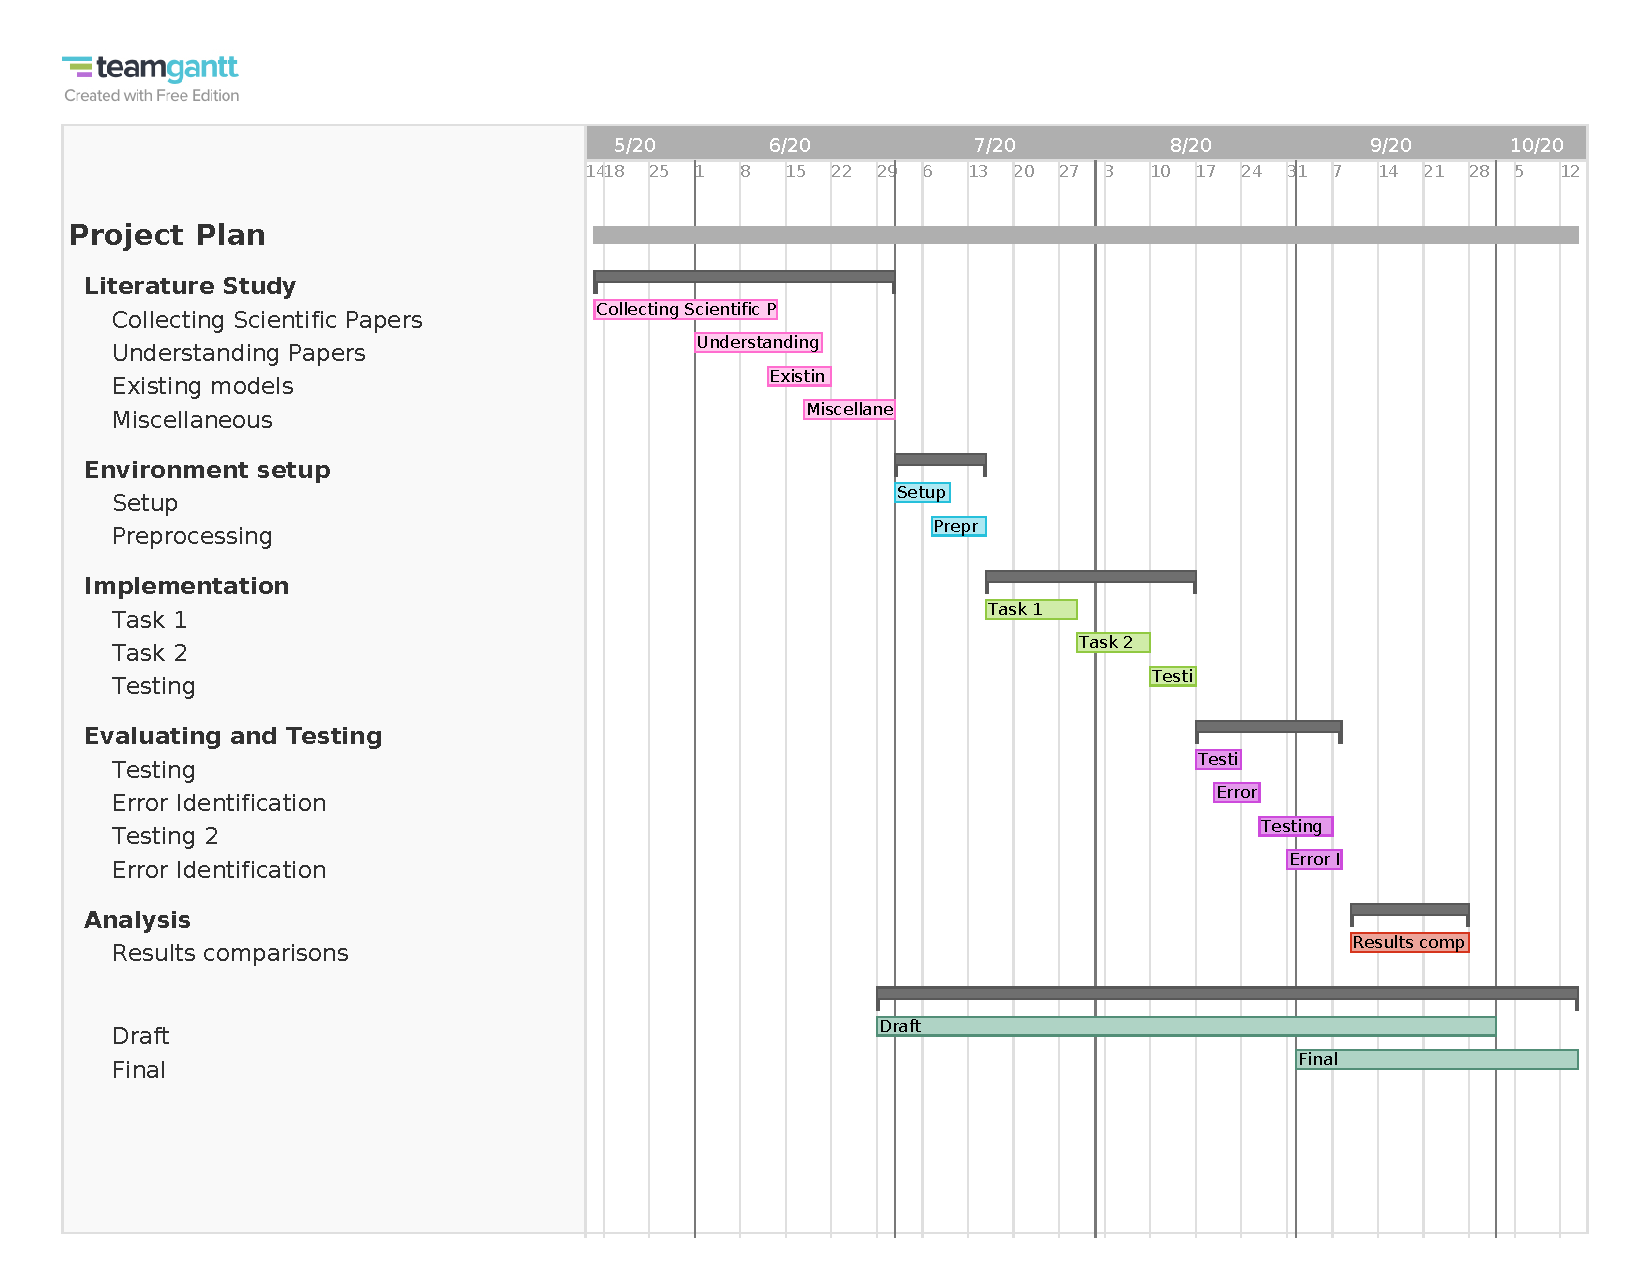
\includegraphics[width=1.0\textwidth]{plan.pdf}
    \caption{Caption}
    \label{fig:plan}
\end{figure}

\newpage
\bibliographystyle{plain}
\bibliography{references.bib}

\end{document}
